%----------------------------------------------------------------------------
\chapter{Összehasonlítás}
%----------------------------------------------------------------------------

	A programot offline módban különböző eszközökön futtatva a futási idejüket hasonlítottam össze.
	A program a kamera képe helyett korábban felvett 1000 darab \texttt{*.raw} nyers fájlokat dolgozott fel.
	A \ref{table:results}. táblázatban látható futási eredmények csupán a kernel időket tartalmazza.
	
	\begin{table}[H]
	\footnotesize
	\centering
	
	\setlength{\extrarowheight}{3pt}
	\begin{tabular}{ l | r | r | r | r}
		 & GTX 330m & Xeon E5-1620 & Xeon PHI & GTX 590\\ \hline
		\texttt{MAX\_COMPUTE\_UNITS} & 6 & 8 & 224 & 16\\
		\texttt{MAX\_CLOCK\_FREQUENCY} & 1265\,MHz & 3000\,MHz & 1100\,MHz & 1225\,MHz\\
		\texttt{MAX\_WORK\_GROUP\_SIZE} & 512 & 8192 & 8192 & 1024\\ \hline\hline
		\texttt{GLOBAL\_MEM\_SIZE} & 1\,Gbyte & 8\,Gbyte & 4.5\,Gbyte & 1.5\,Gbyte\\
		\texttt{MAX\_MEM\_ALLOC\_SIZE} & $\sim$ 0.25\,Gbyte & $\sim$ 8\,Gbyte & $\sim$ 1.5\,Gbyte & $\sim$ 0.4\,Gbyte\\
		\texttt{LOCAL\_MEM\_SIZE} & 16\,Kbyte & 32\,Kbyte & 32\,Kbyte & 48\,Kbyte\\
		\texttt{LOCAL\_MEM\_TYPE} & Local & Global & Global & Local\\\hline
		Futási idő $(T)$ & 114.1~s & 202.0~s & 52.7~s & 7.74~s
	\end{tabular}
	
	\caption[Különböző eszközök futási idejének összehasonlítása]{Az eszközök erőforrásainak és a program futási idejének összehasonlítása.}
	\label{table:results}
	\end{table}
	
	%\usepackage{graphics} is needed for \includegraphics
	\begin{figure}[!h]
	\begin{center}
	  \includegraphics[width=0.9\columnwidth]{figures/eps/runtime.eps}
	  \caption[1000 kép feldolgozásának futási ideje [s].]{1000 kép feldolgozásának futási ideje [s]. A kissebb érték a kedvezőbb.}
	  \label{fig:runtime}
	\end{center}
	\end{figure}
	
	Az eszközök architekturájából fakadó különbségek számszerűsítése végett a futási időt egy compute-unitra és egy
	órajelre fajlagosan számítom:
	\begin{equation}
	T_{\rm fajl} = T \cdot N_{\rm CU} \cdot f_{\rm dev}
	\end{equation}
	ahol $T$ a futási idő $N_{\rm CU}$ az eszköz compute-unit
        száma és $f_{\rm dev}$ az eszköz órajelének frekvenciája. Az
        így definiált $T_{\rm fajl}$ dimenziómentes mennyiség azt
        becsüli meg, hogy az adott feladatot egy compute-unit mennyi
        óraciklus alatt oldaná meg a vizsgált architektúrán.
        
	\begin{table}[H]
	\footnotesize
	\centering
	
	\setlength{\extrarowheight}{3pt}
	\begin{tabular}{ l | r | r | r | r}
		 & GTX 330m & Xeon E5-1620 & Xeon PHI & GTX 590\\ \hline
		\texttt{MAX\_COMPUTE\_UNITS} & 6 & 8 & 224 & 16\\
		\texttt{MAX\_CLOCK\_FREQUENCY} & 1265\,MHz & 3000\,MHz & 1100\,MHz & 1225\,MHz\\\hline\hline
		Futási idő $(T)$ & 114.1~s & 202.0~s & 52.7~s & 7.74~s\\
		Fajlagos futási idő $(T_{\rm fajl})$ & 0.86$\times 10^{12}$ & 4.85$\times 10^{12}$ & 13.00$\times 10^{12}$ & 0.15$\times 10^{12}$
	\end{tabular}
	
	\caption{Eszközök fajlagos futási idejének összehasonlítása}
	\label{table:results_f}
	\end{table}	
	
	%\usepackage{graphics} is needed for \includegraphics
	\begin{figure}[!h]
	\begin{center}
	  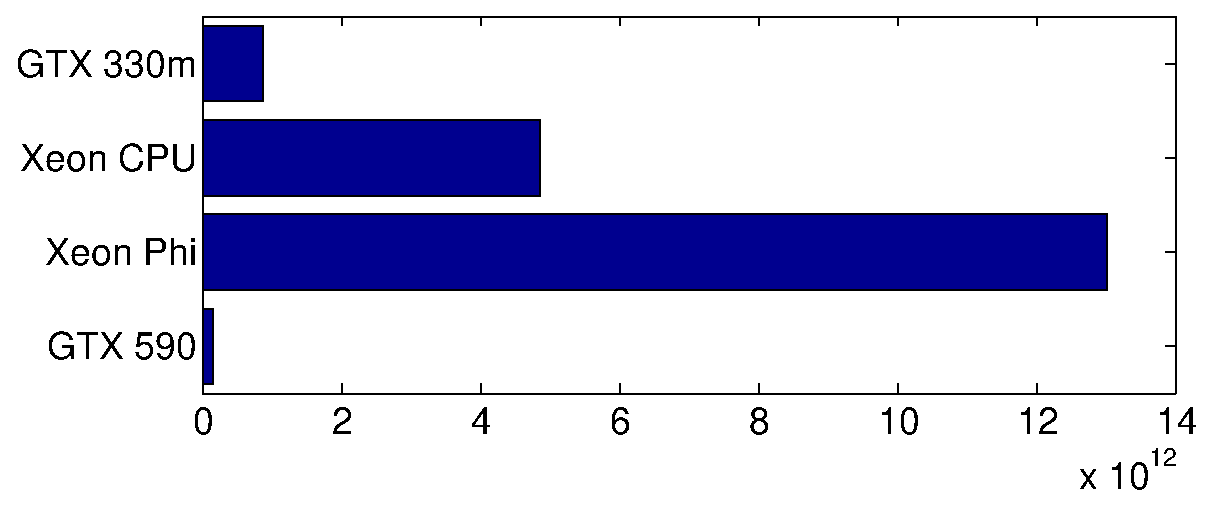
\includegraphics[width=0.9\columnwidth]{figures/eps/runtime_f.eps}
	  \caption[1000 kép feldolgozásának fajlagos futási ideje.]{1000 kép feldolgozásának fajlagos futási ideje. A kissebb érték a
	  kedvezőbb.}
	  \label{fig:runtime_f}
	\end{center}
	\end{figure}
	
	A program OpenCL-ben készült, így videokártyán és processzoron is tud futni.
	Ezt a GPU-k lokális memóriájának és annak programozott ``cache'' működésének pozitív hatásának tudom be.
	
	A \ref{fig:runtime}. ábrát és a \ref{fig:runtime_f}. ábrát összevetve megfigyelhető, hogy a processzorok/processzorkártyák bár
	gyorsabban futtatják a programot, viszont ezt nagy fajlagos idővel teszik. Konklúzióként elmondható, hogy a program
	algoritmusához az architektúrájuk nem illeszkedik.
	
